\documentclass[11pt, letterpaper]{memoir}
\usepackage{HomeworkStyle}
\geometry{margin=0.75in}



\begin{document}

\begin{center}
	{\large Quiz 11.2 -- Rotational Spectroscopy}
\end{center}
{\large Name: \rule[-1mm]{4in}{.1pt}

\subsection*{}
Below is a microwave spectrum of the CN radical

\noindent
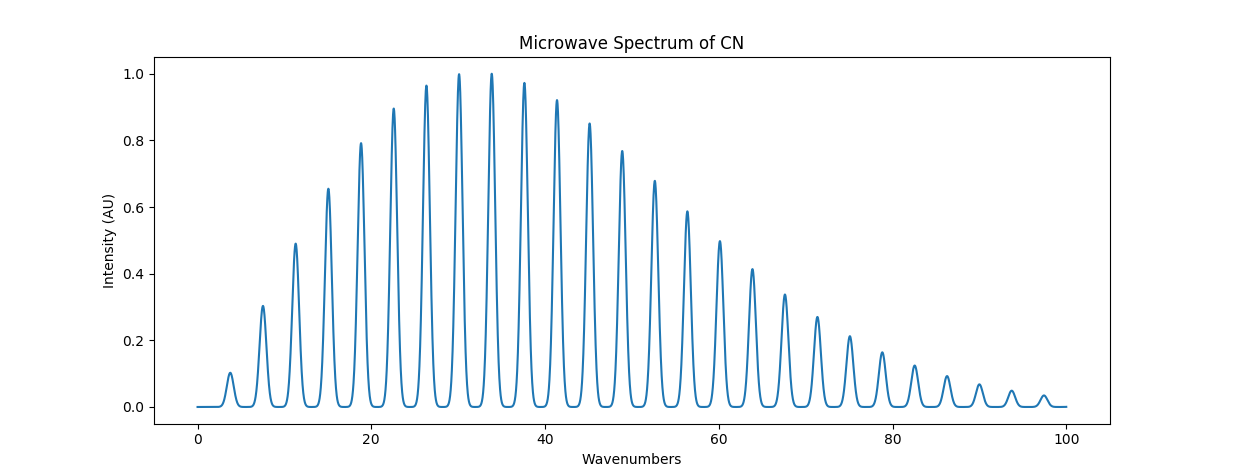
\includegraphics[trim= 0 0 0 0, clip=true, width=\linewidth]{CN_Microwave}

\noindent
Using the spectrum, find the following quantities:
\begin{enumerate}
	\item $\tilde{B}$
	\item $r$ (Bond length)
	\item Temperature
	\item $\tilde{D}_J$
\end{enumerate}

\newpage
\pagestyle{empty}
\addtocounter{page}{-1}
\section*{\emph{{\fontspec{Malgun Gothic}오늘} (Today)}}
\paragraph{By {\fontspec{Malgun Gothic}구상} (Ku Sang)}~

{\fontspec{Malgun Gothic}
\begin{verse}
	오늘도 신비의 샘인 하루를 맞는다.

	이 하루는 저 강물의 한 방울이\\
	어느 산골짝 옹달샘에 이어져 있고\\
	아득한 푸른 바다에 이어져 있듯\\
	과거와 미래와 현재가 하나다.

	이렇듯 나의 오늘은 영원 속에 이어져\\
	바로 시방 나는 그 영원을 살고 있다.

	그래서 나는 죽고 나서부터가 아니라\\
	오늘서부터 영원을 살아야 하고\\
	영원에 합당한 삶을 살아야 한다.

	마음이 가난한 삶을 살아야 한다.\\
	마음을 비운 삶을 살아야 한다.
\end{verse}
}

\vspace{2em}
\begin{verse}
	Today again I meet a day, a well of mystery.

	Like a drop of that river extends to\\
	a spring of a valley and then to\\
	the faraway blue sea, for this day\\
	the past, the future, and the present are one.

	So does my today extend to eternity,\\
	and right now I am living the eternity.

	So, starting from today, I should live\\
	eternity, not after I die,\\
	and should live a life that deserves eternity.

	I should live the life of a poor heart.\\
	I should live the life of an empty heart.
\end{verse}
\end{document}
